	\documentclass[twoside]{article}
\usepackage{../../estilo-ejercicios}
\renewcommand{\baselinestretch}{1,3}
%--------------------------------------------------------
\begin{document}

\title{Tarea 3 de Algorítmica}
\author{Javier Aguilar Martín}
\maketitle


\begin{ejercicio}{Lower Bound for Binary Search}
Supongamos que hemos procesado $n$ elementos formando una lista ordenada. Probar que encontrar un elemento concreto entre ellos en el \emph{Comparison Model} requiere un tiempo $\Omega(\log n)$. 
\end{ejercicio}
\begin{solucion}
Sea $L$ la lista, $L[i]$ el elemento $i$-ésimo y $x$ el elemento que buscamos. Cualquier algoritmo de búsqueda hará comparaciones entre $x$ y los elementos de $L$. Para cada comparación tenemos 3 posibilidades:
\begin{itemize}
\item $x\leq L[i]$. 
\item $x=L[i]$.
\item $x>L[i]$.
\end{itemize}
A partir de estas posibilidades construimos un árbol el árbol de decisión de cualquier algoritmo que parta de un nodo con la comparación de $x$ con un $L[i]$ concreto de la siguiente forma:
\begin{itemize}
\item Si $x\leq L[i]$, crear una rama a la izquierda, donde el primer nodo compara $x$ con el siguiente $L[j]$ que corresponda en el algoritmo y el resto de nodos se construye recursivamente.
\item Si $x=L[i]$ o no hay elementos con los que comparar $x$, el nodo es una hoja.
\item Si $x>L[i]$, crear una rama a la derecha de forma análoga al primer caso. 
\end{itemize}
En el peor caso, esto es, que tenga que el elemento no esté en la lista o que se encuentre en la última comparación, el árbol con menos altura es el que surge de empezar la búsqueda en la mitad de la lista, ya que es el que minimiza la distancia máxima de un elemento de la lista al $L[i]$ de inicio. Esto se puede observar gráficamente, ya que el árbol construido así es aquel en el que cada nodo tiene 2 hijos en todos los casos posibles, y por tanto cualquier otro árbol binario requeriría algún nivel extra para completar todos los nodos (todos los elementos de la lista deberían aparecer en el árbol en el peor caso). Esto es, tenemos un árbol de la siguiente forma, donde FAIL representa que la lista ha terminado sin haber encontrado $x$:

\begin{center}
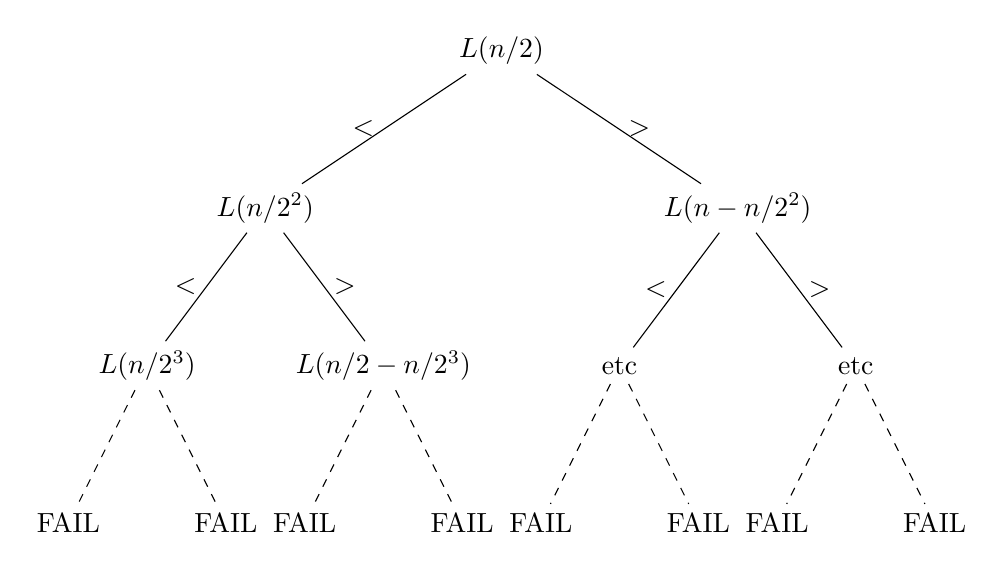
\begin{tikzpicture}[level distance=2cm,
  level 1/.style={sibling distance=6cm},
  level 2/.style={sibling distance=3cm},
  level 3/.style={sibling distance=2cm}]
  \node {$L(n/2)$}
    child {node {$L(n/2^2)$} 
      child {node {$L(n/2^3)$} 
      	child[dashed] {node{FAIL}}
      	child[dashed] {node{FAIL}} edge from parent node[left]{$<$}}
      child {node {$L(n/2-n/2^3)$}
          child[dashed] {node {FAIL}   }
          child[dashed] {node {FAIL} } edge from parent node[right] {$>$}}edge from parent node[left] {$<$}
    }
    child {node {$L(n-n/2^2)$}
    child {node {etc}
     child[dashed] {node {FAIL}}
     child[dashed] {node {FAIL}} edge from parent node[left]{$<$}}
      child {node {etc}
      	child[dashed] {node{FAIL}    }
      	child[dashed] {node {FAIL}}edge from parent node[right] {$>$}}edge from parent node[right] {$>$}
    };
\end{tikzpicture}
\end{center}
%tenemos cota superior porque el binary search de irte al medio y ver si coger la mitad superior o inferior es log(n)

Fijándonos en la rama más a la izquierda observamos que el árbol tiene altura $h$ tal que $2^h=n$, o lo que es lo mismo, $h=\log n$. Esto prueba que el tiempo máximo de ejecución de cualquier algoritmo de búsqueda es $\Omega(\log n)$. 
\end{solucion}



\end{document}
